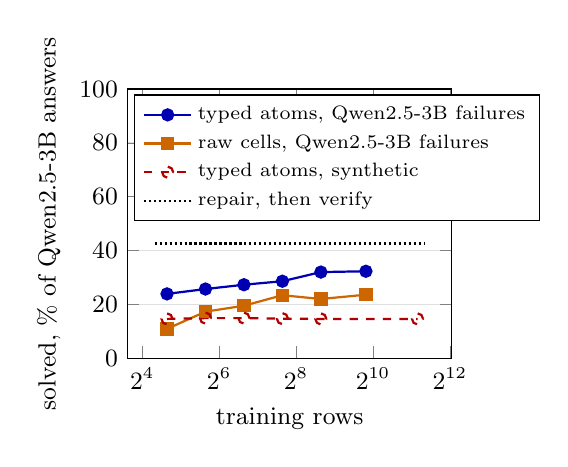
\begin{tikzpicture}
\begin{axis}[width=0.47\linewidth, height=5.0cm, xmode=log, log basis x=2, xlabel={training rows}, ylabel={solved, \% of Qwen2.5-3B answers},
  ymin=0, ymax=100, ymajorgrids, grid style={gray!25}, legend style={font=\scriptsize, at={(0.02,0.98)}, anchor=north west}, legend cell align=left,
  tick label style={font=\small}, label style={font=\small}]
\addplot[blue!70!black, mark=*, thick] coordinates {(25,23.9) (50,25.7) (100,27.3) (200,28.6) (400,32.0) (900,32.3)};
\addlegendentry{typed atoms, Qwen2.5-3B failures}
\addplot[orange!80!black, mark=square*, thick] coordinates {(25,10.9) (50,17.3) (100,19.5) (200,23.4) (400,22.0) (900,23.6)};
\addlegendentry{raw cells, Qwen2.5-3B failures}
\addplot[red!70!black, dashed, mark=o, thick] coordinates {(25,14.6) (50,14.9) (100,14.9) (200,14.7) (400,14.6) (2282,14.6)};
\addlegendentry{typed atoms, synthetic}
\addplot[black, densely dotted, thick, domain=20:2600, samples=2] {42.6};
\addlegendentry{repair, then verify}
\end{axis}
\end{tikzpicture}
